\begin{frame}{Workflow Overview}
	\begin{overlayarea}{\textwidth}{.1\textheight}
    \only<1>{CAD design}
	\only<2>{STL interface}
	\only<3>{Voxelized topology}
	\only<4>{Specification of loads and fixtures}
	\only<5>{Optimized topology}
	\only<6>{Surface extraction}
	\only<7>{Parametrized CAD-geometries}
	\only<8>{Iterative design process}
	\end{overlayarea}
	\begin{overlayarea}{\textwidth}{.9\textheight}
    \begin{center}
		\begin{tikzpicture} 
        \uncover<+->{
        \node at (0,3)[inner sep=0pt](N1)
                {
\includegraphics[width=2cm]{Pictures/1CAD.pdf}};
		}               
        \uncover<+->{
        \node at (3,3) [inner sep=0pt](N2)
                {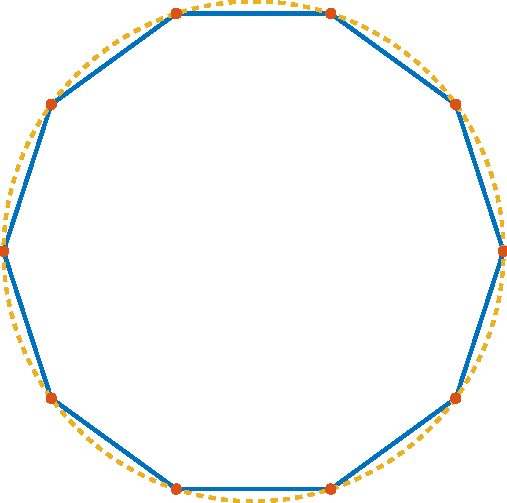
\includegraphics[width=2cm]{Pictures/2STL.pdf}};
        \draw[thick,->] (N1) -- (N2);
        }
        \uncover<+->{
        \node at (6,3)[inner sep=0pt](N3)
                {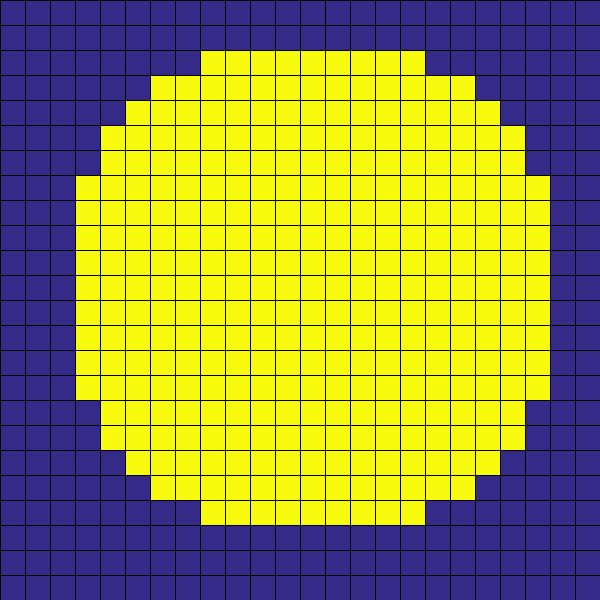
\includegraphics[width=2cm]{Pictures/3VOX.pdf}};
        \draw[thick,->] (N2) -- (N3);
        }
        \uncover<+->{
        \node at (9,1.5)[inner sep=0pt](N4)             
                {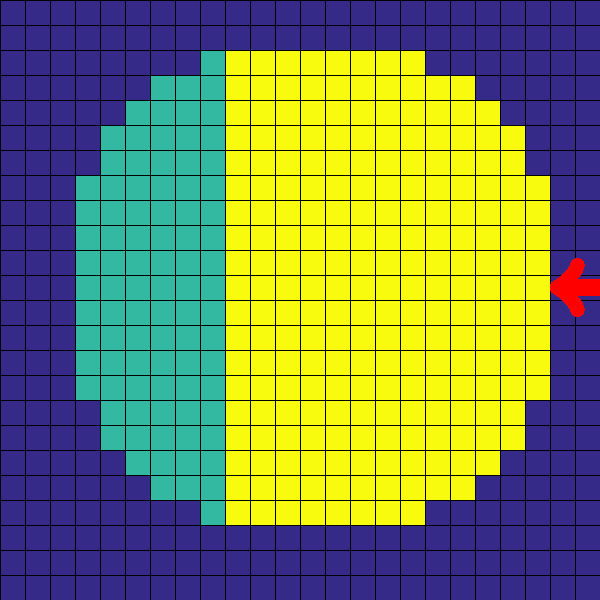
\includegraphics[width=2cm]{Pictures/4TPD.pdf}};
        \draw[thick,->] (N3) -- (N4);
        }
        \uncover<+->{
        \node at (6,0)[inner sep=0pt](N5) 
                {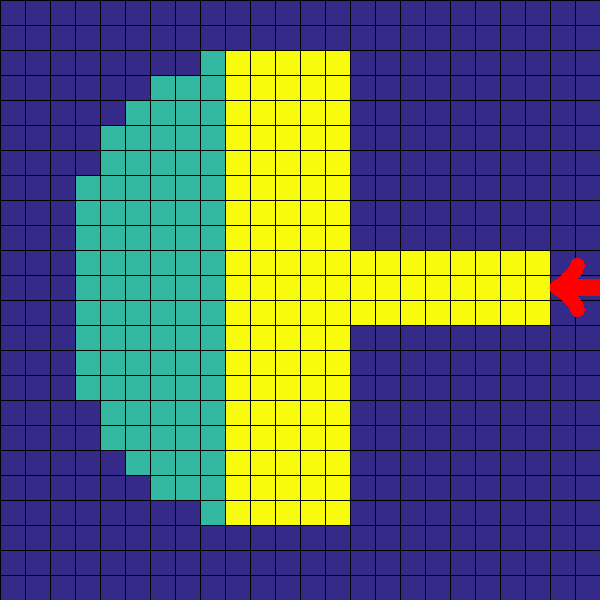
\includegraphics[width=2cm]{Pictures/5TOPOPT.pdf}};
        \draw[thick,->] (N4) -- (N5); 
        }
        \uncover<+->{
        \node at (3,0)[inner sep=0pt](N6)
                {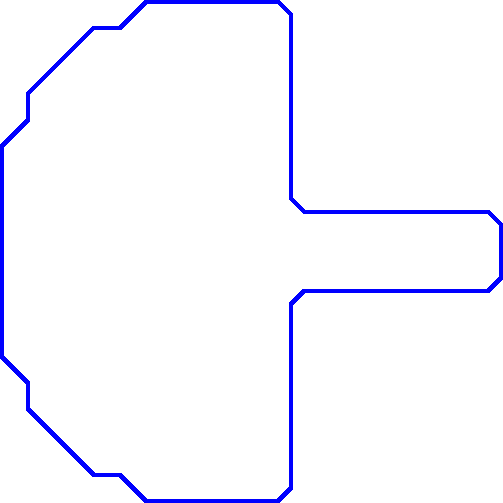
\includegraphics[width=2cm]{Pictures/7MC.pdf}};
        \draw[thick,->] (N5) -- (N6); 
        }
        \uncover<+->{
        \node at (0,0)[inner sep=0pt](N7)
                {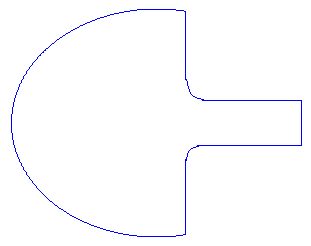
\includegraphics[width=2.2cm,height=2.2cm]{Pictures/End.png}};        
        \draw[thick,->] (N6) -- (N7);                
		}        
        \uncover<+->{
        \draw[thick,->] (N7) -- (N1); 
        }
        \end{tikzpicture}
	\end{center}
	\end{overlayarea}

\end{frame}
